\documentclass[tikz,border=6pt]{standalone}
\usepackage{amsmath}
\usetikzlibrary{arrows.meta,positioning,shapes.geometric}
\begin{document}
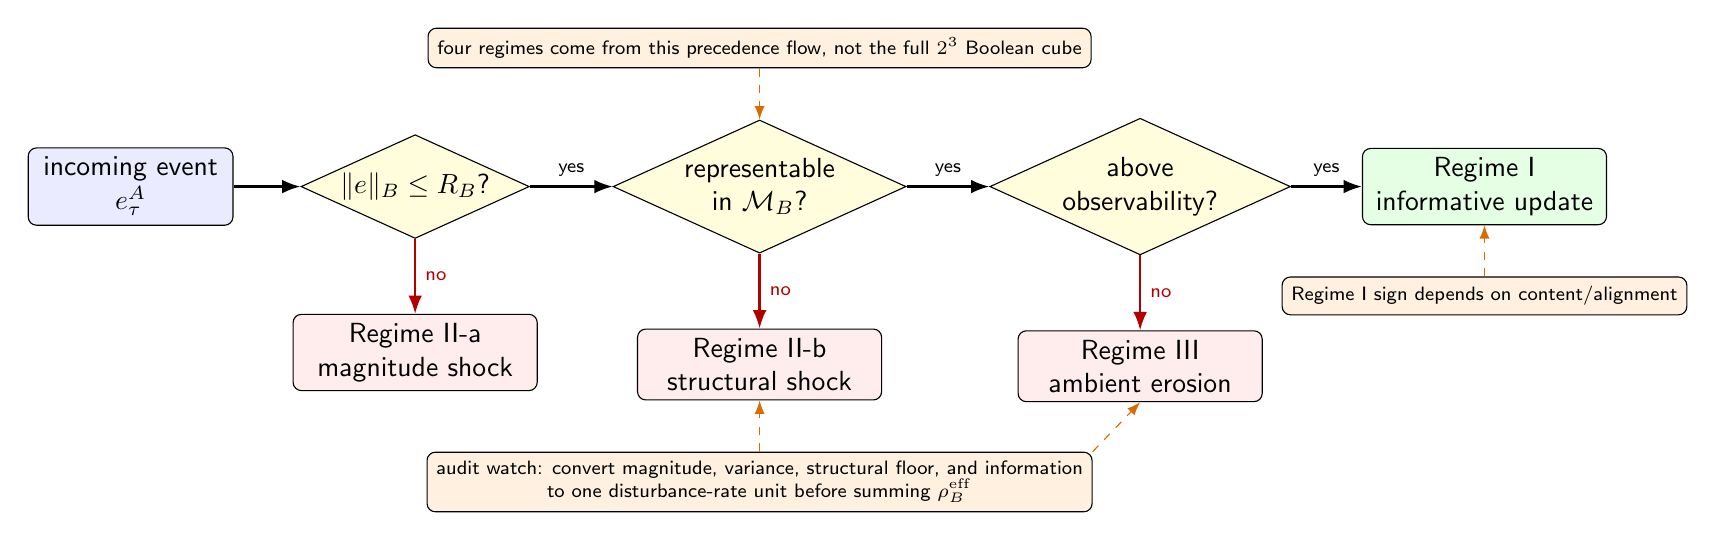
\begin{tikzpicture}[
  font=\sffamily,
  >=Latex,
  start/.style={draw, rounded corners=3pt, fill=blue!8, align=center, minimum width=2.6cm, minimum height=0.75cm},
  test/.style={draw, diamond, aspect=2.2, fill=yellow!14, align=center, inner sep=1pt, minimum width=2.9cm},
  regime/.style={draw, rounded corners=3pt, fill=green!10, align=center, minimum width=3.1cm, minimum height=0.82cm},
  bad/.style={draw, rounded corners=3pt, fill=red!7, align=center, minimum width=3.1cm, minimum height=0.82cm},
  warn/.style={draw, rounded corners=3pt, fill=orange!12, align=center, font=\sffamily\scriptsize}
]

\node[start] (event) {incoming event\\$e^A_\tau$};
\node[test, right=0.85cm of event] (mag) {$\|e\|_B\le R_B$?};
\node[test, right=1.05cm of mag] (class) {representable\\in $\mathcal M_B$?};
\node[test, right=1.05cm of class] (obs) {above\\observability?};
\node[regime, right=0.9cm of obs] (regI) {Regime I\\informative update};

\node[bad, below=0.95cm of mag] (regIIa) {Regime II-a\\magnitude shock};
\node[bad, below=0.95cm of class] (regIIb) {Regime II-b\\structural shock};
\node[bad, below=0.95cm of obs] (regIII) {Regime III\\ambient erosion};

\draw[->, thick] (event) -- (mag);
\draw[->, thick] (mag) -- node[above, font=\sffamily\scriptsize] {yes} (class);
\draw[->, thick] (class) -- node[above, font=\sffamily\scriptsize] {yes} (obs);
\draw[->, thick] (obs) -- node[above, font=\sffamily\scriptsize] {yes} (regI);
\draw[->, thick, red!70!black] (mag) -- node[right, font=\sffamily\scriptsize] {no} (regIIa);
\draw[->, thick, red!70!black] (class) -- node[right, font=\sffamily\scriptsize] {no} (regIIb);
\draw[->, thick, red!70!black] (obs) -- node[right, font=\sffamily\scriptsize] {no} (regIII);

\node[warn, above=0.65cm of class, minimum width=4.2cm] (precedence)
  {four regimes come from this precedence flow, not the full $2^3$ Boolean cube};
\draw[->, dashed, orange!85!black] (precedence.south) -- (class.north);

\node[warn, below=0.65cm of regIIb, minimum width=5.4cm] (units)
  {audit watch: convert magnitude, variance, structural floor, and information\\to one disturbance-rate unit before summing $\rho_B^{\rm eff}$};
\draw[->, dashed, orange!85!black] (units.north) -- (regIIb.south);
\draw[->, dashed, orange!85!black] (units.north east) -- (regIII.south);

\node[warn, below=0.65cm of regI, minimum width=3.6cm] (sign)
  {Regime I sign depends on content/alignment};
\draw[->, dashed, orange!85!black] (sign.north) -- (regI.south);

\end{tikzpicture}
\end{document}
